\begin{figure*}[t]
    \centering
    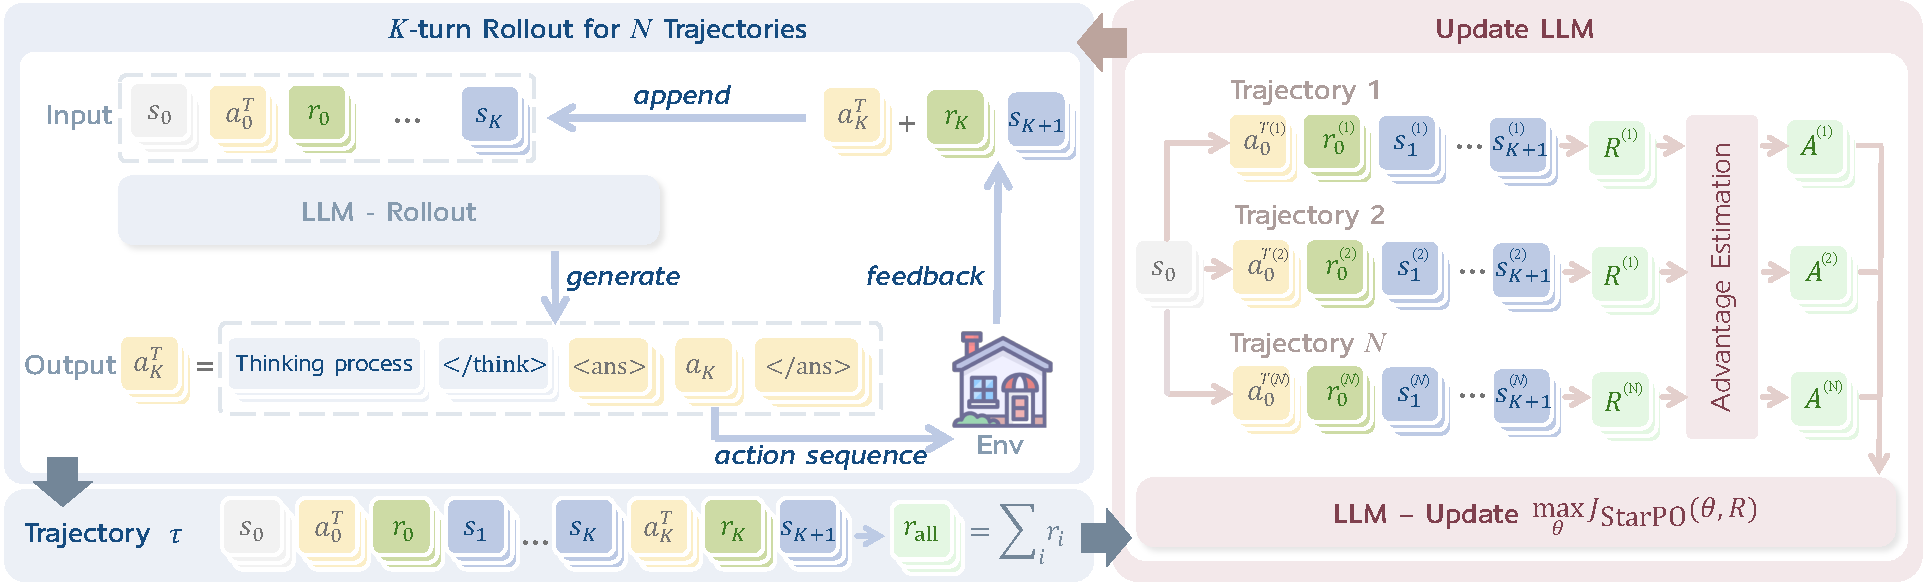
\includegraphics[width=\textwidth]{figures/starpo.pdf}
    \caption{\small The State-Thinking-Actions-Reward Policy Optimization (StarPO) framework. LLM generates reasoning-guided actions for multi-turn interactions with environments and accumulates trajectory-level rewards, normalized and used to update the LLM policy.}
    \label{fig:starpo}
    \vspace{-5pt}
\end{figure*}

\section{Framework}

\subsection{The MDP Formulation for Agent Training}

Previous reinforcement learning (RL) for language models often assumes a single-turn setting, where the goal is to maximize the expected reward $R(s, a)$ over prompt-response pairs $(s, a)$ sampled from a dataset $\mathcal{D}$:
\begin{equation}
    J_{\text{step}}(\theta) = \mathbb{E}_{s \sim \mathcal{D}, a \sim \pi_\theta(\cdot|s)}[R(s, a)].
\end{equation}

However, LLM-based agents must operate in interactive environments that unfold over multiple turns and exhibit stochastic feedback. To capture these dynamics, we formulate the problem as a Markov Decision Process (MDP) $\mathcal{M} = \{S, A, P\}$, where
$S$ represents states (e.g., observation sequences or interaction histories), $A$ represents actions (often token sequences), and $P$ denotes the transition dynamics and reward generation process. The agent policy $\pi_\theta$ generates an action $a_t$ at each time step $t$, conditioned on the current state $s_t$ and the interaction history. The environment returns a reward $r_t$ and a new state $s_{t+1}$ given the current transition dynamics:
\[
    a_t \sim \pi_\theta(\cdot | s_t, \tau_{<t}), \quad (r_t, s_{t+1}) \sim P(\cdot | s_t, a_t),
\]
where $\tau_{<t} = \{s_0, a_0, r_0, ..., s_{t-1}, a_{t-1}, r_{t-1}\}$ denotes the interaction history. This interactive process continues for a maximum horizon $K$, yielding a full trajectory $\tau = \{s_0, a_0, r_0, ..., s_K\}$ that forms the learning material for the agent.

\subsection{StarPO: Reinforcing Reasoning via Trajectory-Level Optimization}

We introduce \textbf{StarPO} (State-Thinking-Action-Reward Policy Optimization), a general RL framework designed to optimize entire multi-turn interaction trajectories for LLM agents. Unlike previous methods for static tasks that treat each action independently, StarPO treats the \textbf{entire trajectory}—including observations, reasoning traces, actions, and feedback—as a coherent unit for rollout and model optimization.
The objective is to maximize expected trajectory reward:
\begin{equation}
    J_{\text{StarPO}}(\theta) = \mathbb{E}_{\mathcal{M}, \tau \sim \pi_{\theta}} \left[R(\tau) \right],
\end{equation}
where $\mathcal{M}$ is the MDP, $\tau$ is a full sequence of reasoning-augmented interactions, and $R(\tau)$ denotes the cumulative reward over the entire trajectory. The policy probability $\pi_\theta(\tau)$ is decomposed into token-level likelihoods, making StarPO directly compatible with autoregressive LLMs. Figure~\ref{fig:starpo} illustrates the full StarPO process, and we break them down in detail below.

\definecolor{bgcolor}{RGB}{232, 236, 240} 
\definecolor{badgecolor}{RGB}{181, 192, 208}  
\begin{onebox}{Trajectory-Level Objective in StarPO vs. Previous Methods}
\textbf{Previous methods (e.g., PPO~\citep{schulman2017proximalpolicyoptimizationalgorithms}, GRPO~\citep{shao2024deepseekmathpushinglimitsmathematical}):}
\[
\textcolor{black}{
J_{\text{step}}(\theta) = \mathbb{E}_{x \sim \mathcal{D},\, y \sim \pi_\theta(\cdot|x)}\left[ R(x, y) \right]
}
\quad
\textcolor{gray}{
\text{(optimize single-turn output } y \text{ given input } x)
}
\]

\textbf{StarPO (ours):}
\[
\textcolor{red!80!black}{
J_{\text{StarPO}}(\theta) = \mathbb{E}_{\mathcal{M}, \tau \sim \pi_\theta}\left[ R(\tau) \right]
}
\quad
\textcolor{red!80!black}{
\text{(optimize total reward over trajectory } \tau = \{s_0, a_0, r_0\dots, s_K\})
}
\]
\end{onebox}


\subsubsection{Optimization Procedure: Learning from Reasoning-Interaction Trajectories}

At each training iteration, the agent begins from an initial state $s_0$ and generates $N$ trajectories. At each step $t$, the agent produces a reasoning-guided structured output:
\begin{equation}
    a^T_t = \texttt{<think>}...\texttt{</think><answer>}~a_t~\texttt{</answer>},
\end{equation}
where $a^T_t$ is the full action output including intermediate reasoning, and $a_t$ is a sequence of environment-executable sub-action. The environment then returns the next state $s_{t+1}$ and reward $r_t$. The rollout stage produces complete trajectories $\tau = \{s_0, a^T_0, r_0, s_1, ..., a^T_{K-1}, r_{K-1}, s_K\}$, where \textit{every component is LLM-generated or environment-induced} and will be jointly optimized.

StarPO interleaves rollout and update steps.
% , supporting both online and offline learning modes.
New rollouts can be generated on-policy using $\pi_\theta$, or sampled from a replay buffer under $\pi_{\text{old}}$.
% This enables StarPO to flexibly unify online RL, offline RL, and hybrid training setups.
Each training loop consists of $P$ initial states $s_0$, each generating $N$ trajectories, and updates are performed with batch size $E$ for $L$ total loops. This yields $S = \frac{L \cdot P \cdot N}{E}$ total gradient update steps. Additional training mechanisms are discussed in \S\ref{sec:exp}.


\subsubsection{Modular Optimization Strategies}

StarPO supports a variety of policy optimization algorithms under a unified trajectory-level abstraction. For each rollout trajectory $\tau_i = \{\tau_{i,(1)}, \ldots, \tau_{i,(|\tau_i|)}\}$ of totally $|\tau_i|$ tokens, we instantiate StarPO with the following optimization strategies for token-level updates:
\vspace{-5pt}
\begin{itemize}[left=2pt, itemsep=2pt, topsep=4pt]
    \item \textbf{PPO~\citep{schulman2017proximalpolicyoptimizationalgorithms}.} We use the PPO objective (More details can be found in Appendix~\ref{app:a.rl}), where a critic is trained to estimate token-level value and advantages $A_{i,t}$:
    \begin{equation}
    \small
        J_{\text{PPO}}(\theta) = \frac{1}{G} \sum_{i=1}^G \frac{1}{|\tau_i|} \sum_{t=1}^{|\tau_i|}
        \min \left[
            \frac{\pi_\theta(\tau_{i,(t)}|\tau_{i,<t})}{\pi_{\text{old}}(\tau_{i,(t)}|\tau_{i,<t})} \cdot A_{i,t},\,
            \text{clip}\left( \frac{\pi_\theta(\tau_{i,(t)}|\tau_{i,<t})}{\pi_{\text{old}}(\tau_{i,(t)}|\tau_{i,<t})}, 1 - \epsilon, 1 + \epsilon \right) \cdot A_{i,t}
        \right],
    \end{equation}
    where $G$ is the number of trajectories in the batch, $\tau_{i,(t)}$ denotes the $t$-th token in trajectory $\tau_i$, and $\tau_{i,<t}$ is its prefix.

    \item \textbf{GRPO~\citep{shao2024deepseekmathpushinglimitsmathematical}.} For critic-free training leveraging GRPO, we assign a scalar reward $R(\tau_i)$ to each trajectory and normalized advantage $\hat{A}_{i,t}$ across all tokens in $\tau_i$:
    \begin{equation}
    \small
        \hat{A}_{i,t} = \frac{R(\tau_i) - \text{mean}(\{R(\tau_1), \ldots, R(\tau_G)\})}
                             {\text{std}(\{R(\tau_1), \ldots, R(\tau_G)\})}.
    \end{equation}
    The GRPO objective becomes:
    \begin{equation}
        \small
        J_{\text{GRPO}}(\theta) = \frac{1}{G} \sum_{i=1}^G \frac{1}{|\tau_i|} \sum_{t=1}^{|\tau_i|} 
        \min \left[
            \frac{\pi_\theta(\tau_{i,(t)}|\tau_{i,<t})}{\pi_{\text{old}}(\tau_{i,(t)}|\tau_{i,<t})} \cdot \hat{A}_{i,t},\,
            \text{clip}\left( \frac{\pi_\theta(\tau_{i,(t)}|\tau_{i,<t})}{\pi_{\text{old}}(\tau_{i,(t)}|\tau_{i,<t})}, 1 - \epsilon, 1 + \epsilon \right) \cdot \hat{A}_{i,t}
        \right].
    \end{equation}
\end{itemize}


\subsection{The RAGEN System}

To implement StarPO in practice, we build \textbf{RAGEN}, a complete system for LLM agent training in controlled environments. RAGEN supports structured rollouts, customizable reward functions, and integration with multi-turn, stochastic environments. It serves both as the execution backend for StarPO and as a platform for studying stability, generalization, and learning dynamics in training reasoning agents.
RAGEN is designed to be extensible: new environments, reward schemes, or rollout  strategies can be easily plugged in, serving as a foundation for RL-based agent training.


% \subsubsection{Modular Optimization Strategies}

% StarPO supports a variety of policy optimization algorithms by unifying them under a trajectory-centric RL abstraction. Given a rollout trajectory $\tau$ collected using the old policy $\pi_{\text{old}}$, the general optimization objective is:
% \begin{equation}
%     J_{\text{StarPO}}(\theta) = \mathbb{E}_{\tau \sim \pi_{\text{old}}, P} \left[ \frac{\pi_\theta(\tau)}{\pi_{\text{old}}(\tau)} R(\tau) \right],
% \end{equation}
% where $R(\tau)$ is the trajectory-level reward and $\pi_\theta(\tau) = \prod_i \pi_\theta(\tau_{(i)}|\tau_{(<i)})$ is the full token-level likelihood under the new model.

% We instantiate this general objective with the following optimization strategies:

% \begin{itemize}
%     \item \textbf{PPO.} We estimate token-level advantages $A_i$ using a value function over trajectories. The PPO objective becomes:
%     \begin{equation}
%         J_{\text{PPO}}(\theta) = \mathbb{E}_{\tau, i} \left[ \min \left( r_i(\theta) A_i, \text{clip}(r_i(\theta), 1-\epsilon, 1+\epsilon) A_i \right) \right],
%     \end{equation}
%     where $r_i(\theta) = \frac{\pi_\theta(\tau_{(i)}|\tau_{(<i)})}{\pi_{\text{old}}(\tau_{(i)}|\tau_{(<i)})}$ is the per-token likelihood ratio.

%     \item \textbf{GRPO.} For critic-free training, we assign normalized scalar rewards to the full trajectory and optimize:
%     \begin{equation}
%         J_{\text{GRPO}}(\theta) = \mathbb{E}_{\tau \sim \pi_{\text{old}}} \left[ \frac{\pi_\theta(\tau)}{\pi_{\text{old}}(\tau)} \cdot \tilde{R}(\tau) \right],
%     \end{equation}
%     where $\tilde{R}(\tau)$ is a normalized version of $R(\tau)$ (e.g., across rollout batch or history buffer).
%     TODO: add original GRPO formula from DSMath paper
%     TODO: Unify Actions/Action in StarPO
% \end{itemize}

% This formulation enables fair comparisons across optimization methods and unifies online and offline learning under a single trajectory-aware framework.



% \section{RAGEN Framework}
% \subsection{The MDP formulation for Agent Training}
% For simple, single-turn tasks, the RL goal is to maximize the expected reward $R(s, a)$ over the dataset $\mathcal{D}$ by generating a response $a$ to a prompt $s$ from a policy $\pi_\theta$:
% \begin{equation}
% J(\theta) = \mathbb{E}_{s \sim \mathcal{D}, a \sim \pi_\theta(\cdot|s)}[R(s, a)].
% \end{equation}
% However, agent tasks involve multi-turn interactions and environmental stochasticity. We model RL on agent tasks with Markov Decision Processes (MDPs, \citet{mdp}), such that $\mathcal{M} = \{S, A, P\}$. In the LLM agent settings, states $S$ and actions $A$ are token sequences and $P$ denotes environmental dynamics of state change and reward distribution. The agent's policy $\pi_\theta$ chooses actions $a_t \sim \pi_\theta(\cdot|s_t, [s, a, r]_{0:t-1})$ leading to reward $r_t$ and new states $s_{t+1} \sim P(\cdot|s_t, a_t)$. The objective is to maximizing the expected cumulative reward over the entire interaction trajectory:
% \begin{equation}
%     J_{\text{Interactive}}(\theta) = \mathbb{E} _{(r_t, s_{t+1}) \sim P(\cdot|s_t, a_t), a_t \sim \pi_\theta(\cdot|s_t, [s,a,r]_{0:t-1})}\left[ \sum_t r(s_t, a_t) \right],
%     \label{eq:interactive}
% \end{equation}
% where $r(s_t,a_t)$ is the reward obtained at the $t^{\rm th}$ turn. This trains agents to optimize for long-term goals in the dynamic environments.
% \subsection{StarPO: Reinforcing Reasoning in Agent Training}
% The key challenge in optimizing $J_{\rm{interactive}}$ lies in enforcing reasoning across multiple turns with RL, without relying on Supervised Fine-Tuning (SFT) data. 
% This is particularly challenging in multi-turn agent settings -- reasoning should be done on the entire future trajectories while maintaining computationally efficient policy updates. 
% Building on the success of rule-based RL in curating explicit \texttt{<think>} processes to emerge reasoning~\citep{deepseekai2025deepseekr1incentivizingreasoningcapability}, we investigate whether LLMs can develop similar reasoning capabilities in multi-turn interactions. 
% Inspired by policy optimization algorithms like SARSA~\citep{rummery1994line}, PPO~\citep{schulman2017proximalpolicyoptimizationalgorithms} and GRPO~\citep{shao2024deepseekmathpushinglimitsmathematical}, we propose \textbf{State-Thinking-Actions-Reward Policy Optimization} (StarPO), which effectively optimize LLM policy $\pi_{\theta}$, maximizing $J_{\rm{interactive}}$ and facilitate effective and stable reasoning-guided agent training.
% StarPO enables (1) learning LLM policy $\pi_{\theta}$ to optimize the entire trajectory $\tau$, jointly optimizing
% state changes, reasoning and action strategy, and (2) train LLMs with normalized trajectory rewards for \textbf{stable} policy optimization.
% As shown in Figure~\ref{fig:starpo}, StarPO alternates between \textit{Rollout} and \textit{Update} phases:
% \noindent\textbf{Rollout Stage: Reasoning-Interaction Chain Generation.} ~
% In the Rollout stage, given an initial state  $s_0$ from environment distribution $P$, the LLM generates $N$ trajectories $\{\tau\}_{N}$, each up to $K$ turns. As shown in Figure~\ref{fig:starpo} (Left), at each step $t$, the model processes the trajectory:
% \begin{equation}
%    \tau_{1:t-1} = \langle s_0, a^T_0, r_0, s_1, ..., s_{t-1}, a^T_{t-1}, r_{t-1}, s_{t}\rangle,
% \end{equation}
% and generates an reasoning-guided action sequence:
% \begin{equation}
%     a^T_t= \texttt{<think>...</think><answer>} a_t \texttt{</answer>}.
% \end{equation}
% Here, $a^T_t$ represents the thinking-augmented action and $a_t=[a_{t_1}, a_{t_2}, ...]$ is an \textbf{action sequence} under the environment action space $A$.
% The environment processes $a_t$ action-by-action and returns \textbf{feedback} consisting of the accumulative reward $r_t = \sum_{i} r(s_{t_i},a_{t_{i+1}})$ and the starting state for the next turn $s_{t+1}=s_{t_{|a_t|}}$, which are appended to $\tau_{1:t-1}$ for the next step LLM generation. We detail the design of $r_t$ of each environment in \S\ref{sec:exp}, which include both task-wise reward and format-wise reward to reinforce reasoning and decision-making processes. 
% \noindent\textbf{Update Stage: Multi-turn Trajectory Optimization. }~
% As shown in Figure~\ref{fig:starpo} (Right), after the rollout stage we obtain trajectories $\{\tau\}_{N}$ generated by LLM. Then, we train LLMs on these trajectories to optimize $J_{\rm interactive}(\theta)$ in Eq.~\ref{eq:interactive}. Inspired by the success of rule-based RL~\citep{deepseekai2025deepseekr1incentivizingreasoningcapability}, we rely not on costly Supervised Fine-Tuning (SFT) data but design reward functions by adapting single-turn rule-based reward function to multi-turn trajectory-level optimization. Considering the trajectory prediction requires a long-horizon global understanding and LLMs have potential environment dynamic modeling capabilities, rather than following a step-by-step interactive format as $J_{\rm{interactive}}(\theta)$ in Eq. \ref{eq:interactive}, we optimize the entire trajectory as:
% \begin{equation}
%     J_{\rm{StarPO}}(\theta) = \mathbb{E}_{\substack{(r_t, s_{t+1}) \sim P(\cdot|s_t, a_t),a_t \sim \pi_{old}(\cdot|s_t, [s,a,r]_{0:t-1})}}\left[\frac{\pi_\theta(\tau)}{\pi_{\text{old}}(\tau)}R(\tau)\right],
% \end{equation}
% where the trajectories $\tau$ are generated using the old model's policy and environment dynamics (i.e., $a_t \sim \pi_{\text{old}}, (r_t, s_{t+1})\sim P$) while the trajectory-level probability $\pi(\tau)$ is calculated through token-level probability $\prod_i \pi(\tau_{(i)}|\tau_{(<i)})$, where $\tau_{(i)}$ are the $i$-th LLM token rather than interaction turn. To support an online learning approach, we continuously set the old policy to the model immediately after update during training. $R(\tau)$ is a surrogate reward assigned to the trajectory $\tau$. Details on the reward function $r$ can be found in \S\ref{subsec:reward}.
% For experimental settings, each loop of StarPO has a prompt size $P$ (each with different initial states $s_0$). The LLM generates trajectories of rollout size $N$ each prompt, and is updated with an update batch size of $E$ and number of loops $L$. This leads to total gradient update steps $S=\frac{L\cdot N\cdot P}{E}$.
% \subsection{Rule-Based Reward Modeling}
% \label{subsec:reward}
% Recently, Group-Relative Policy Optimization methods~\citep{liu2025DRGRPO, shao2024deepseekmathpushinglimitsmathematical} demonstrates the potential efficacy of rule-based reward modeling over actor-critic algorithms~\cite{haarnoja2018softactorcritic, schulman2017proximalpolicyoptimizationalgorithms} in providing stable reward signal for efficient RL training. In this work, we conduct a detailed examination of these methodologies, focusing on two critical factors for rule-based reward modeling: \textbf{grouping strategy} and \textbf{normalization function}.
% Instances within the same group are jointly considered for normalization, and normalization function determines treatment of instances inside a group for LLM policy weight updates.
% \noindent\textbf{Grouping Strategy. }~
% To maximize simplicity while processing trajectory-level rewards, StarPO evaluates a multi-turn trajectory $\tau$ with trajectory-level reward $R(\tau)$ computed by summing up rewards across steps $r(\tau)$, then grouped through different followed by normalization functions. 
% We denote the accumulative reward for a trajectory $\tau$ as $r(\tau) = \sum_t\tau_{r_t}$, where $r(\tau)$ denotes accumulative reward in trajectory $\tau$ and $\tau_{r_t}$ denotes the $t$-th step reward $r_t$ in trajectory $\tau$. We explore three progressive grouping strategy with various group sizes:
% \vspace{-5px}
% \begin{itemize}
%     \item \textbf{State-level Grouping}: Normalizes rewards within trajectories from the same initial state $s_0$. Each trajectory $\tau_{i,j}$ are assigned to group $G_i = \{\tau_{i,1}, \tau_{i,2}, \ldots, \tau_{i,N}\}$ for reward normalization.
%     \item \textbf{Batch-level Grouping}: Considers all trajectories in a batch collectively. For a batch with $B$ prompts each generating $N$ trajectories, we create a single group $G = \{\tau_{1,1}, \tau_{1,2}, \ldots, \tau_{B,N}\}$ and normalize rewards across this entire batch.
%     \item \textbf{Inductive Grouping}: Dynamically partitions trajectories based on inductive information, clustering them into subgroups $\{G_k\}$ for more nuanced reward normalization.
% \end{itemize}
% \vspace{-5px}
% \noindent\textbf{Normalization Function. }~
% After grouping trajectories, we apply normalization functions to convert raw rewards into learning signals:
% \vspace{-5px}
% \begin{itemize}
% \item \textbf{Z-score Normalization}~\citep{shao2024deepseekmathpushinglimitsmathematical}: Standardizes rewards to have zero mean and unit variance:
% \begin{equation}
%     R_z(\tau) = \frac{r(\tau) - \mu_G}{\sigma_G + \epsilon}
% \end{equation}
% where $\mu_G$ is the mean reward in group $G$, $\sigma_G$ is the standard deviation, and $\epsilon$ is a small constant to prevent division by zero. This normalization accounts for both the mean and variance of rewards, making it suitable for groups with different reward distributions.
% \item \textbf{Mean Subtraction Normalization}~\citep{liu2025DRGRPO}: Centers the rewards around zero by subtracting the group mean:
% \begin{equation}
%     R_m(\tau) = r(\tau) - \frac{1}{|G|}\sum_{\tau' \in G}r(\tau')
% \end{equation}
% This approach focuses on relative performance compared to the group average, enabling the model to learn from trajectories that exceed mean performance.
%  \item \textbf{Asymmetric Min-Clip Normalization}: Inspired by~\cite{yu2025DAPO}, we design asymmetric normalization function to reward solving difficult problems while not excessively penalizing failures on simpler tasks:
%     \begin{equation}
%         R_a(\tau) = \text{clip}\left(\frac{r(\tau) - \mu_G}{\sigma_G + \epsilon}, \gamma, +\infty\right)
%     \end{equation}
%     where $\gamma <0$ is a lower bound that clips negative rewards, preventing excessive penalties. This straightforward approach maintains strong positive rewards for solving difficult problems while establishing a minimum threshold for penalties, encouraging risk-taking on challenging tasks without overly punishing failures.
% \end{itemize}
% \vspace{-5px}








% We explore three progressive normalization strategies~\citep{henderson2019deepreinforcementlearningmatters} to stablize reward signals taking different aspects of RL training. Empirical analysis are detailed in \S\ref{sec:abgrpo}.
% \subsubsection{Absolute Reward Policy Optimization}
% Absolute Reward Policy Optimization (ARPO) is the simplest approach that preserves raw rewards:
% \begin{equation}
%     R^{\rm{ARPO}}(r_{\rm all}^{(i)}) = r_{\rm all}^{(i)},
% \end{equation}
% where $r_{\rm all}^{(i)}$ denotes the overall reward obtained in the $i^\text{th}$ trajectory. ARPO provides consistent measurements across training, but struggles in unstable reward scale environments (e.g. Sokoban).
% \subsubsection{Batch-Relative Policy Optimization}
% Batch-Relative Policy Optimization (BRPO) normalizes rewards across each training batch:
% \begin{equation}
%     R^{\rm{BRPO}}(r_{\rm all}^{(i)}) = (r_{\rm all}^{(i)} - \mu_B)/\sigma_B.
% \end{equation}
% The BRPO normalization maintains steady reward scales independent of environments, and adapts to model capabilities by a) amplifying positive rewards when $\mu_B$ is low, and b) increasing penalties when performance improves, providing better focus across different training stages.
% \subsubsection{Group-Relative Policy Optimization}
% Group-Relative Policy Optimization (GRPO) \citep{shao2024deepseekmathpushinglimitsmathematical}
% normalizes in prompt groups to handle varying difficulties for different problems:
% \begin{equation}
%     R^{\rm{GRPO}}(r_{\rm all}^{(i)}) = (r_{\rm all}^{(i)} - \mu_{p_i})/\sigma_{p_i}.
% \end{equation}
% The GRPO normalization balances learning across tasks by adapting to prompt complexity, providing stronger reinforcement for success on difficult prompts while penalizing failures on simpler ones.
% To summarize, each normalization has specific purposes: ARPO keeps simplicity, BRPO adapts to learning progress, and GRPO handles task diversity, jointly enabling effective policy optimization.

% Considering agent tasks introduce multi-turn interactions and environmental stochasticity, 
% we formulate the agent-environment interaction as Markov Decision Processes $\mathcal{M}$ (MDPs, \citet{mdp}), such that $\mathcal{M} = \{S, A, \mathcal{P}\}$. In the LLM agent settings, state space $S$, and action space $A$ are token sequences, enabling LLMs to reason over environment dynamics. At time $t$, state $s_t$ is  transitioned to state $s_{t+1}$ through action $a_t$, following
% \begin{equation*}
% s_{t+1} \sim \mathcal{P}(\cdot|s_t, a_t), 
% \end{equation*}
% where $\mathcal{P}$ is the transition function\footnote{In this paper, we focus on fully observable environments. In partially observable environments such as robotic environments, our formulation can also be easily adapted to a Partially Observable MDP (POMDP, \citet{kaelbling1998planning}) where $o_{t+1} \sim \mathcal{O}(\cdot|s_{t+1}, a_t)$ and $\mathcal{O}$ is the observation function.}.
% The policy $\pi_\theta$ generates actions given the trajectory:
% \begin{equation*}
% a_t \sim \pi_\theta(\cdot|s_t, [s, a]_{0:t-1}).
% \end{equation*}
% Based on this formulation, the objective of multi-turn step-by-step interactions becomes:
% % \begin{align*}
% % &J_{\rm{Interactive}}(\theta) 
% % = \mathbb{E}_{\pi_\theta}[\sum_{t} r(s_t, a_t)].
% % \end{align*}
% \begin{equation}
%     J_{\rm{Interactive}}(\theta) = \mathbb{E}_{\substack{s_t \sim \mathcal{D} \\ a_t \sim \pi_{\theta}(\cdot|s_t)}}[\sum_{t} r(s_t,a_t)],
%     \label{eq:interactive}
% \end{equation}
